\chapter{Generace X a Y jako spotřebitelé}

Výzkum centra Pew Research Center zjistil, že většina příslušníků každé generace je přesvědčena o své jedinečné, charakteristické identitě\cite[s. 22]{bergh2012coolznacky}.
Marketing se zabývá zjišťováním a naplňováním lidských a společenských potřeb.\cite[s. 43]{kotler2007marketingmanagement} Aby mohl být marketing vůbec úspěšný, je klíčové tuto identitu odhalit.
Jak ukazuje obrázek č. \ref{fig:us-population-by-generation}, generace X a Y souhrnně zastávají nejpočetnější zastoupení v současné populaci. Obě tyto generace mají nicméně jiné hodnoty, rozdílné životní priority, volný čas tráví odlišným způsobem, liší se ve formě komunikace mezi sebou atd. Z pohledu marketingu se tedy chovají jinak i jako spotřebitelé.
Cílem této kapitoly je podat ucelené srovnání těchto dvou skupin jako konzumentů a zjistit, jak se chovají jako zákazníci.

\medskip
\begin{figure}[htbp!]
    \centering
    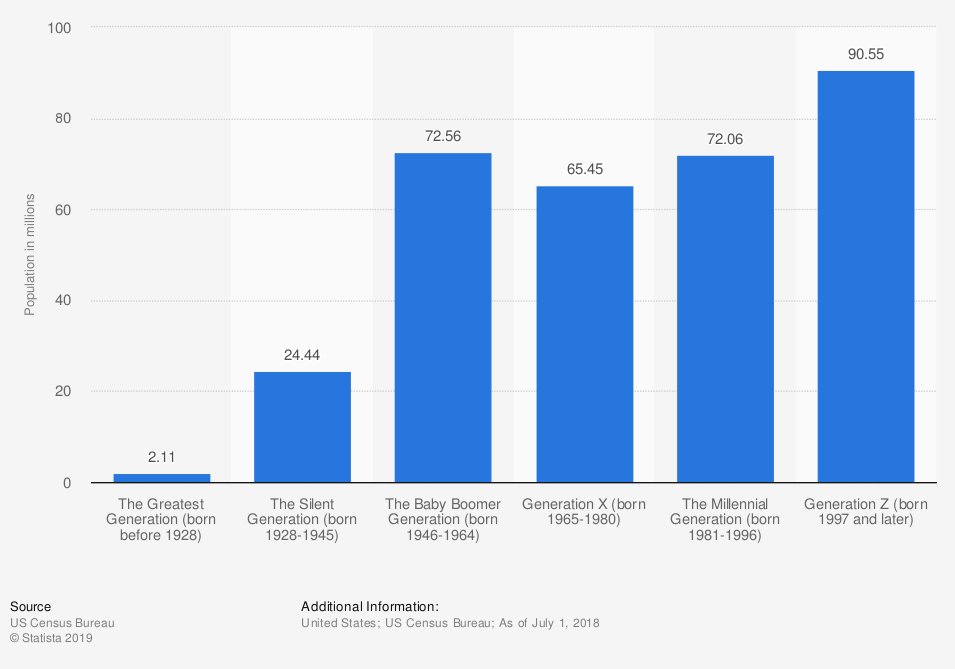
\includegraphics[width=.88\textwidth]{assets/us-population-by-generation.png}
    \caption[Populace US podle generace]{Populace US podle generace \\ Zdroj: Statista.com\protect\footnotemark~podle dat z US Census Bureau }
    \label{fig:us-population-by-generation}
\end{figure}

\footnotetext{Dostupné z: \url{https://www.statista.com/statistics/797321/us-population-by-generation/ }}

\section{Základní priority}
„Generace X byla svědkem kontrastu pracovního světa bez počítačů a příchodem technologií a digitálních inovací. Hodně porovnávají a dokážou ocenit rozsah a dopad těchto inovací, proto upřednostňují organizace, které „myslí dopředu“ a sledují aktuální technologické trendy,“ vysvětluje Ladislav Kučera v rozhovoru na téma \uv{pět generací zaměstnanců}.\cite{idnes2018generacezamestancu} Dále pak zdůrazňuje důraz generace X na rovnováhu mezi soukromým a pracovním životem - mají zodpovědnost za rodinu, děti. Tato generace je více než kterákoli jiná ochotna slevit ze svých mzdových nároků, jsou-li jí nabídnuty jiné výhody, jako je flexibilní pracovní doba, dovolená navíc, zdravotní péče a možnost pracovat z domova.

O generaci mileniálů pak personalista Ladislav Kučera prohlašuje: „Tato věková skupina je považována za zvlášť vytrvalou, ambiciózní, která se nebojí ve své kariéře trochu riskovat. Chce od svého zaměstnavatele slyšet konstruktivní zpětnou vazbu, očekává postup v rámci své role a společnosti“. (tamtéž)
Mileniálové nechtějí být omezováni hranicemi. Jsou si vědomi svých příležitostí a chtějí cestovat a získávat zahraniční zkušenosti.

\section{Média a sociální sítě}
Pro potřeby marketingu je nezbytně nutné šířit povědomí o značce a zvolit vhodné médium s ohledem na cílové zákazníky (reklama a místo jsou ostatně, jak bylo uvedeno, dvě ze čtyř P marketingu).
Přestože generace X se může jevit jako nihilistická a velmi individuálně zaměřená, podle časopisu Forbes má 81\rm \% této generace účet na Facebooku nebo jiné sociální síti\cite{forbes2019generationX} (údaj pro generaci Y sice neuvádějí, ale pravděpodobně bude přinejmenším stejně vysoké). Rozdíl ovšem je v tom, jak a jak často tyto sociální sítě využívají a jakou jim přikládají informační hodnotu.


\medskip
\begin{figure}[htbp!]
    \centering
    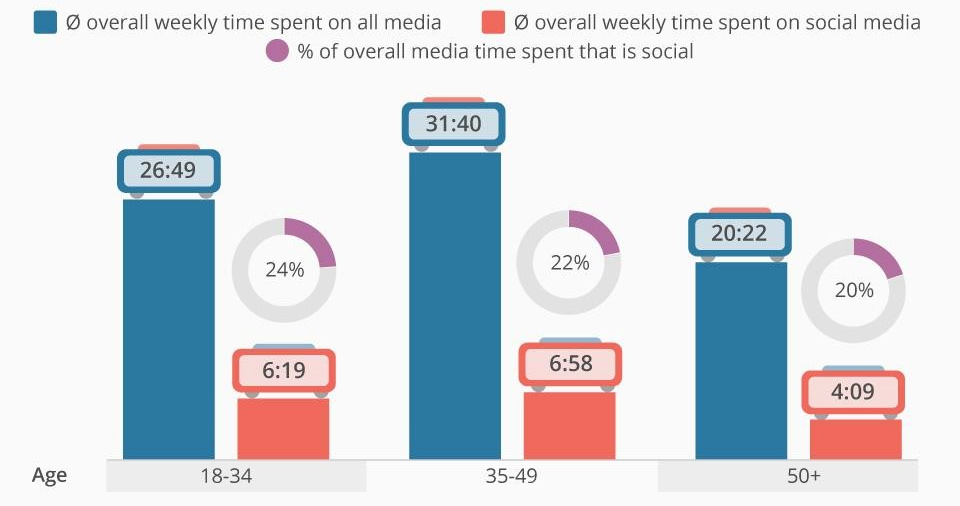
\includegraphics[width=.88\textwidth]{assets/gen-xy-time-spend-on-social-media.png}
    \caption[Porovnání času stráveného na sociálních sítích]{Porovnání času stráveného na sociálních sítích \\ Zdroj: The World Bank\protect\footnotemark }
    \label{fig:cas-na-socialnich-sitich}
\end{figure}

\footnotetext{Dostupné z: \url{http://web.worldbank.org/archive/website01603/WEB/MEDIA-31.HTM}}

Jak je vidět na obr. \ref{fig:cas-na-socialnich-sitich}, generace X tráví více času na médiích (včetně sociálních), než generace Y a to dokonce v řádu hodin. Toto lze vysvětlit např. způsobem, jakým mileniálové využívají svá mobilní zařízení. Analýzou více než 40 tisíc měsíčních účtů za telefon zjistila společnost Nielsen, že američtí teenageři odeslali v průměru \numprint{3146} textových zpráv za měsíc, což je asi 10 zpráv za hodinu v bdělém stavu a mimo školu.\cite[s. 33]{bergh2012coolznacky} Z dalšího výzkumu provedeného společností Deloitte\footnote{Dostupné z \url{https://blog.rescuetime.com/screen-time-stats-2018/}} vyplývá, že průměrně mileniálové kontrolují svůj telefon 58 krát za den, přičemž 70\rm \% těchto interakcí trvá méně než 2 minuty. Jiná studie dodává, že 1 z 10 teenagerů kontroluje svůj telefon alespoň jednou za 4 minuty\footnote{Dostupné z \url{https://nypost.com/2017/11/08/americans-check-their-phones-80-times-a-day-study}}.

Převedeno do marketingového kontextu, reklama cílená na generaci Y by měla být velmi krátká a měla by zaujmout okamžitě, jinak bude ignorována. Generace X bude klást větší důraz na její kvalitu a informační hodnotu.

Dále je velmi užitečné si uvědomit, jakou informační hodnotu médiím jednotlivé generace přidělují. Ve výzkumu provedeném společností eMarketer bylo zjištěno, že 82\rm \% věří tištěným reklamám nebo televizní či rádiové inzerci, zatímco pouhých 42\rm \% má důvěru ve výrobky či produkty, které jsou předmětem reklamy na sociální síti.\footnote{Dostupné z \url{https://www.emarketer.com/Article/Consumer-Trust-Evolving-Digital-Age/1014959}}


\section{Branding}
Moderní spotřebitelé jsou k novým či pro ně neznámým produktům skeptičtí a obvykle prvním krokem, než se rozhodnou pro koupi produktu, je vyhledání komentářů. Jak bylo podotknuto dříve v této práci, informace se v dnešní době šíří prakticky okamžitě a dohledat si je je velmi snadné. To dává do rukou spotřebitelů obrovskou moc a značky si tak musí být vědomy faktu, že i jedno potenciálně špatné hodnocení (byť neoprávněné) může odradit masu potenciálních zákazníků.
V průzkumu InSites Consulting zpracovali studii, ve které se dotazovaných ptali, který zdroj názorů je pro ně při rozhodování o koupi nových kusů oblečení nejdůvěryhodnější. Celkem 74\rm \% respondentů uvedlo, že je pro ně nejdůležitější názor jejich vrstevníků.\cite[s. 43]{bergh2012coolznacky}
Dalším negativním faktorem zejména pro mileniály pak může být neetické chování nebo špatný ekologický dopad. Mileniálové jsou uvědomělí spotřebitelé a problematika ochrany životního prostředí je stále palčivější. Demokratizaci zažívá ochrana planety obecně a pro generaci Y je typické, že se chce aktivně zapojovat a vytvářet vlastní hodnoty.

\subsection{Ztotožnění se se značkou}

Zatímco baby boomers generace si potrpěla na preciznost a kvalitu, pro generaci X a Y jsou mnohem důležitější hodnoty jako dobrá pověst (přitažlivost pro skupinu vrstevníků), kreativita a zábavnost a pravděpodobně nejdůležitější ze všech -- ztotožnění se se značkou. Značky a výrobky, které mladí kupují, se stávají jedním z ústředních bloků, s jejichž pomocí budují svou identitu. Vybírají si značky, se kterými se ztotožňují a které je charakterizují --- mileniálové obecně vykazují jisté formy narcismu, označovaného jako \uv{kampaň na sebe sama} --- a tím zboží dostává symbolickou hodnotu. Neslouží už jen jako nástroj a prostředek, ale zejména jako znak zastupující uvažování a hodnoty nositele.\cite{bergh2012coolznacky}

\subsection{Aakerův model}
Znalost značky sestává ze všech myšlenek, pocitů, představ, zkušeností, přesvědčení atd., které jsou spojovány se značkou. Značky musí u zákazníků především vytvářet silné, příznivé a jedinečné asociace.\cite[s. 315]{kotler2007marketingmanagement}
Příkladem může být společnost Volvo (bezbečnost), Hallmark (starostlivost), Apple (luxus).

Aaker, bývalý profesor marketingu na UC-Berkeley, pohlíží na hodnotu značky jako na soubor pěti kategorií aktiv a pasiv spojených se značkou\cite{kotler2007marketingmanagement}:
\begin{itemize}
    \item věrnost značce
    \item znalost značky
    \item vnímaná kvalita
    \item asociace spojované se značkou
    \item jiná duševní aktiva, např. patenty a obchodní známky
\end{itemize}

Jedinečný soubor asociací pak podle Aakera vytváří identitu značky sestávající se z 12 hledisek jak je ukazuje obr. \ref{fig:aaker-brand-identity-model}.

\medskip
\begin{figure}[htbp!]
    \centering
    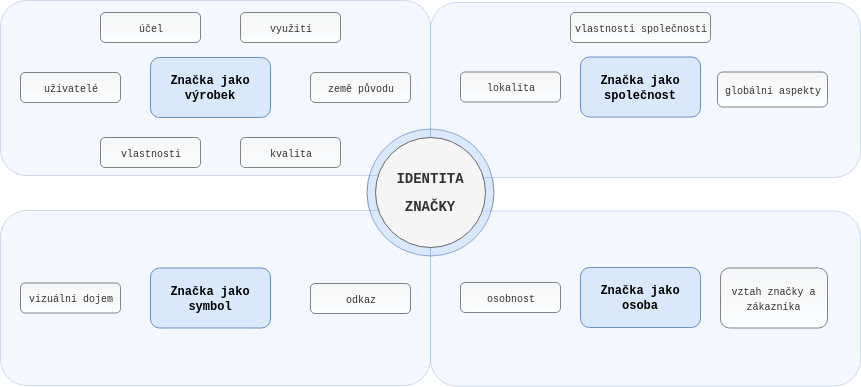
\includegraphics[width=.95\textwidth]{assets/aaker-model.png}
    \caption[Aakerův model identity značky]{Aakerův model identity značky \\ Zdroj: vlastní}
    \label{fig:aaker-brand-identity-model}
\end{figure}

\subsection{Loayalita ke značce}